\documentclass[border=10pt]{standalone}
\usepackage{pgfplots}
\pgfplotsset{compat=1.18}
\pgfplotsset{trig format plots=rad}
\begin{document}
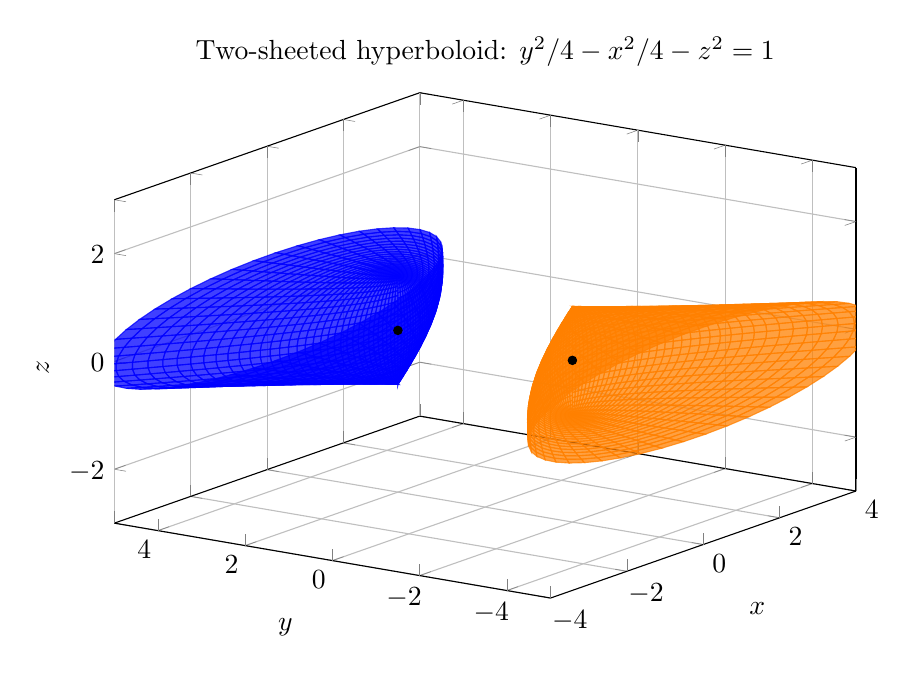
\begin{tikzpicture}
\begin{axis}[
    width=11cm,
    height=8cm,
    xlabel=$x$,
    ylabel=$y$,
    zlabel=$z$,
    title={Two-sheeted hyperboloid: $y^2/4-x^2/4-z^2=1$},
    view={-55}{22},
    xmin=-4, xmax=4,
    ymin=-5, ymax=5,
    zmin=-3, zmax=3,
    grid=major,
    colormap={twosheet}{color=(orange) color=(blue)}
]
\addplot3[
    surf,
    domain=0:1.55,
    y domain=0:2*pi,
    samples=35,
    samples y=50,
    shader=flat,
    opacity=0.75,
    color=blue
]
({2*sinh(x)*cos(y)}, {2*cosh(x)}, {sin(y)});

\addplot3[
    surf,
    domain=0:1.55,
    y domain=0:2*pi,
    samples=35,
    samples y=50,
    shader=flat,
    opacity=0.75,
    color=orange
]
({2*sinh(x)*cos(y)}, {-2*cosh(x)}, {sin(y)});

\addplot3[only marks, mark=*, mark size=1.5pt, black] coordinates {(0,2,0) (0,-2,0)};
\end{axis}
\end{tikzpicture}
\end{document}